%%%%%%%%%%%%%%%%%%%%%%%%%%%%%%%%%%%%%%%%%%%%%%%%%%%%%%%%%%%%%%%%%%%%%%%%%%%%%%%%%
%
% John's part
%
%%%%%%%%%%%%%%%%%%%%%%%%%%%%%%%%%%%%%%%%%%%%%%%%%%%%%%%%%%%%%%%%%%%%%%%%%%%%%%%%%
\section{LOL}% To vanish after the other parts are done ! 
\subsection{Invalidation}
\begin{frame}{Invalidation}
Issues which the pixels from the final depth image won't contain any estimations :
\begin{itemize}
\item Oculusions
\item Saturation of infrared sensors
\item low signal noise ratio
\end{itemize}
How limits this errors ?
\begin{itemize}
\item an algorithms does an invalidation pass durint the post-processing step
\end{itemize}
\end{frame}

\begin{frame}{Invalidation}
\begin{figure}
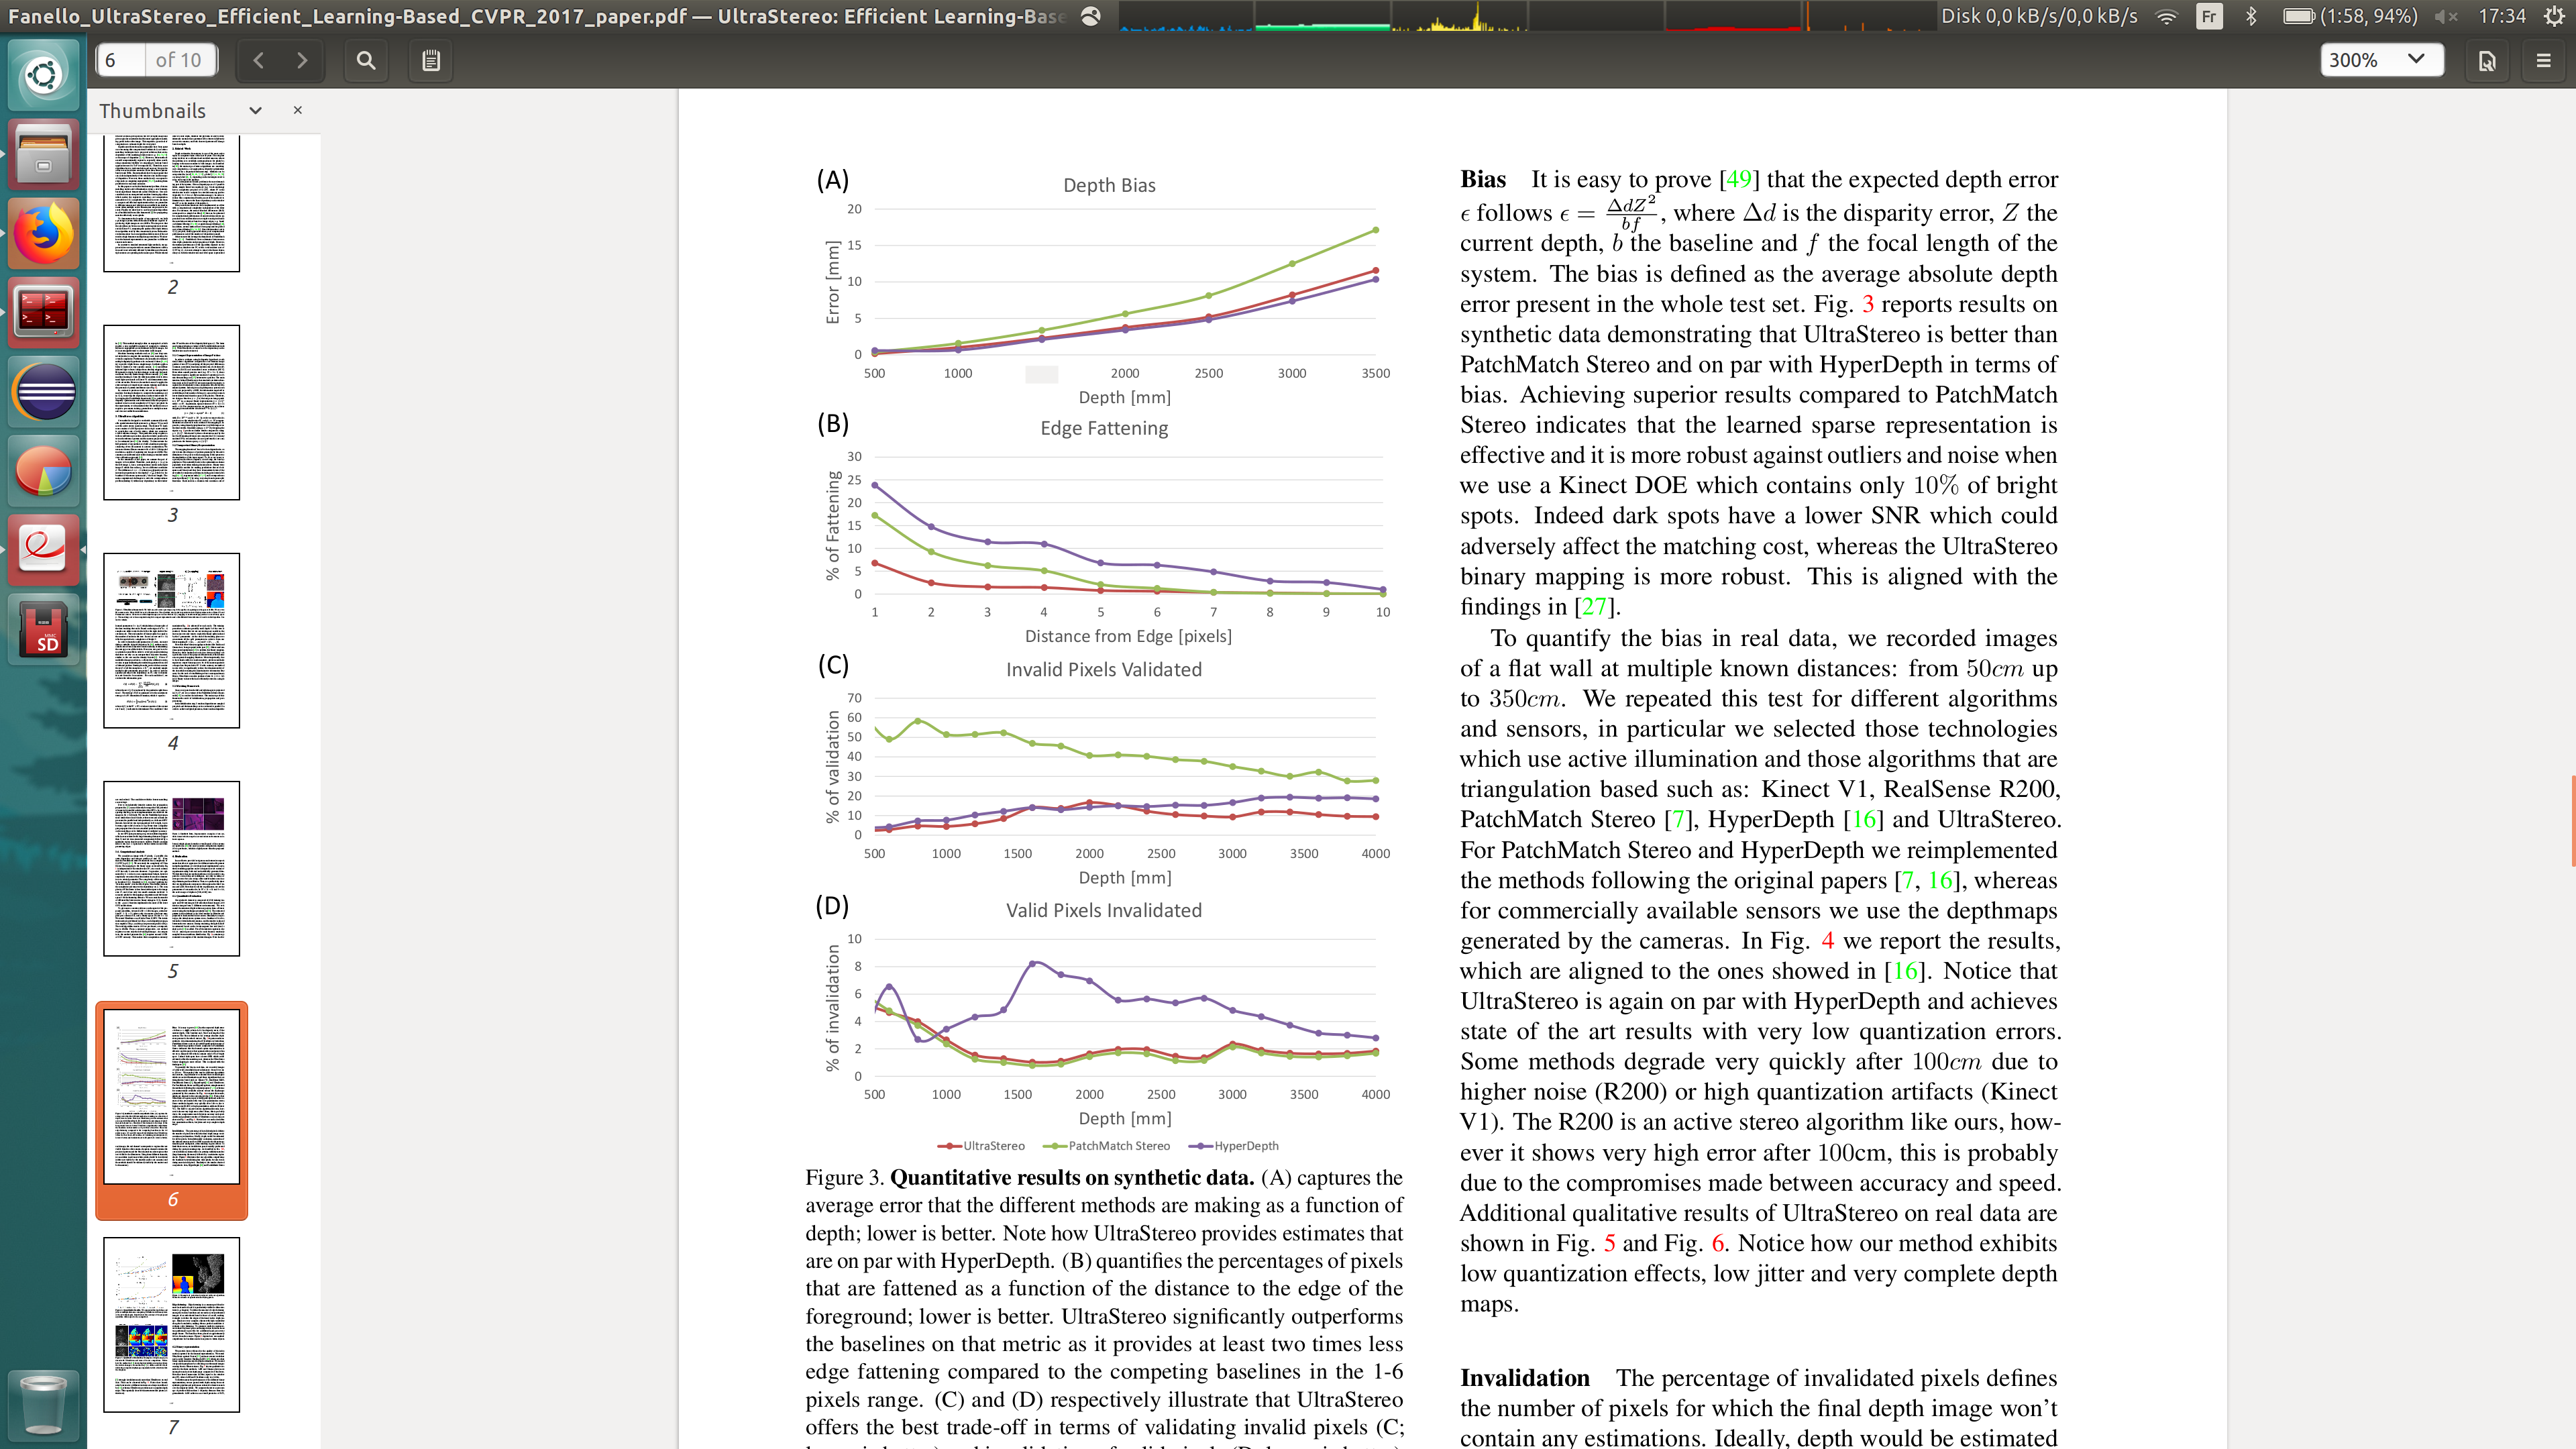
\includegraphics[scale=0.06]{pictures/fig3}
\caption{Quantitative results on syntatic data}
\end{figure}
\end{frame}

\begin{frame}{Example of depth-map produced with UltraStereo}
Look at the thin structures like plants
\begin{figure}
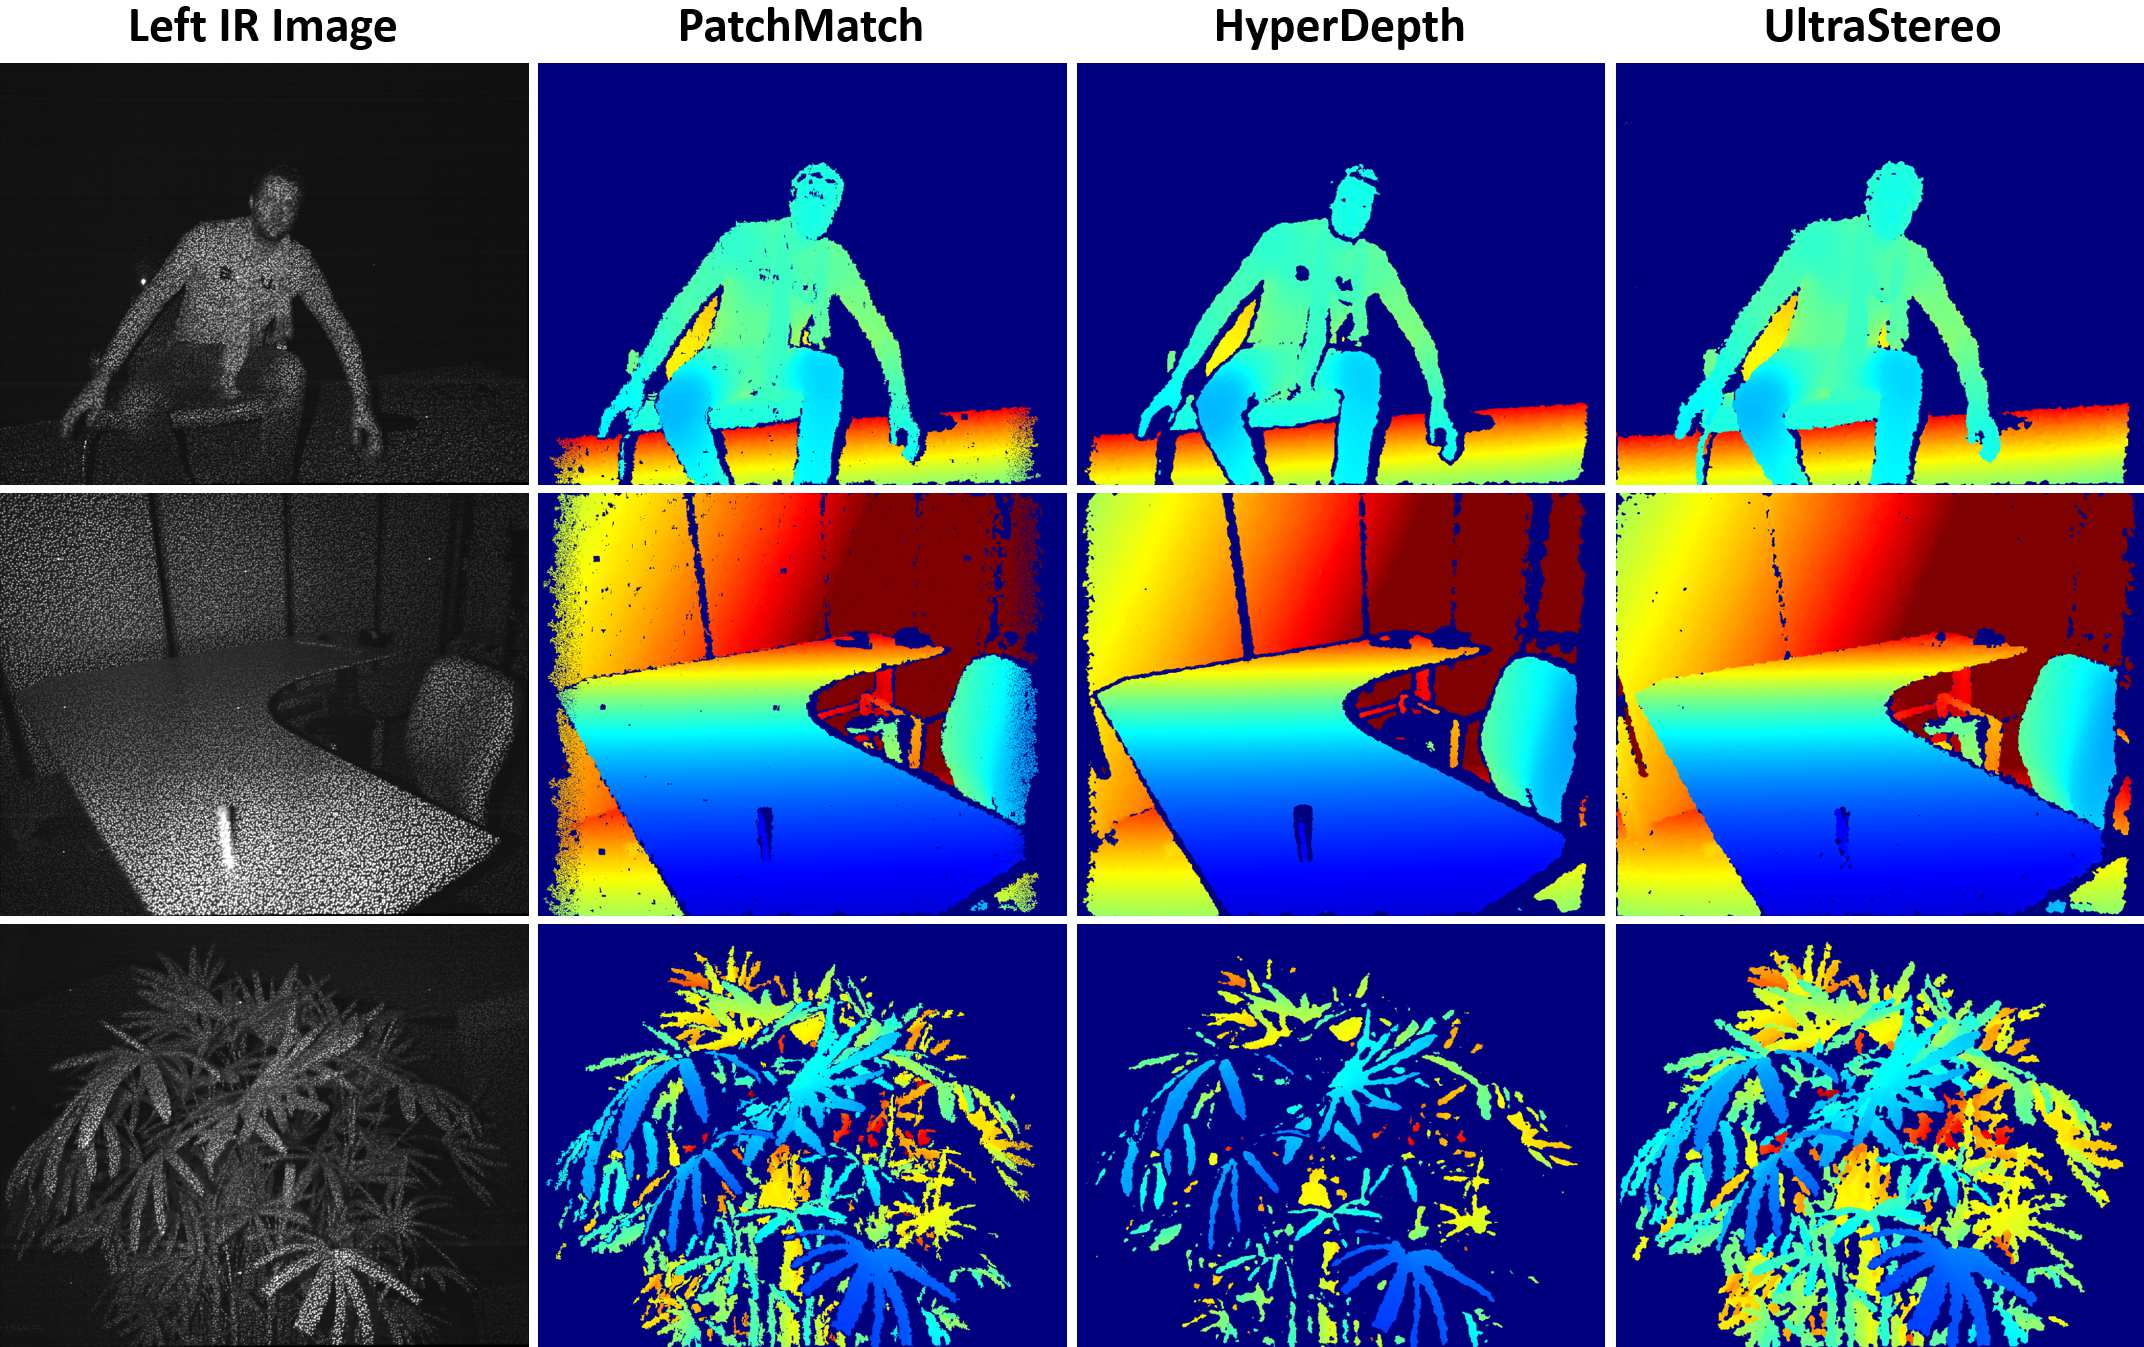
\includegraphics[scale=0.08]{pictures/fig5}
\caption{Qualitative Evaluation}
\end{figure}
\end{frame}

\begin{frame}{Edge fattening}
Other issiue is the edge fattening. To measure it they :
\begin{itemize}
\item used a hand to test their algorithms
\item put a hand at 1 m from the sensors
\item defined key hand pose for each frame
\end{itemize}
\end{frame}

\begin{frame}{Edge fattening}

\begin{figure}
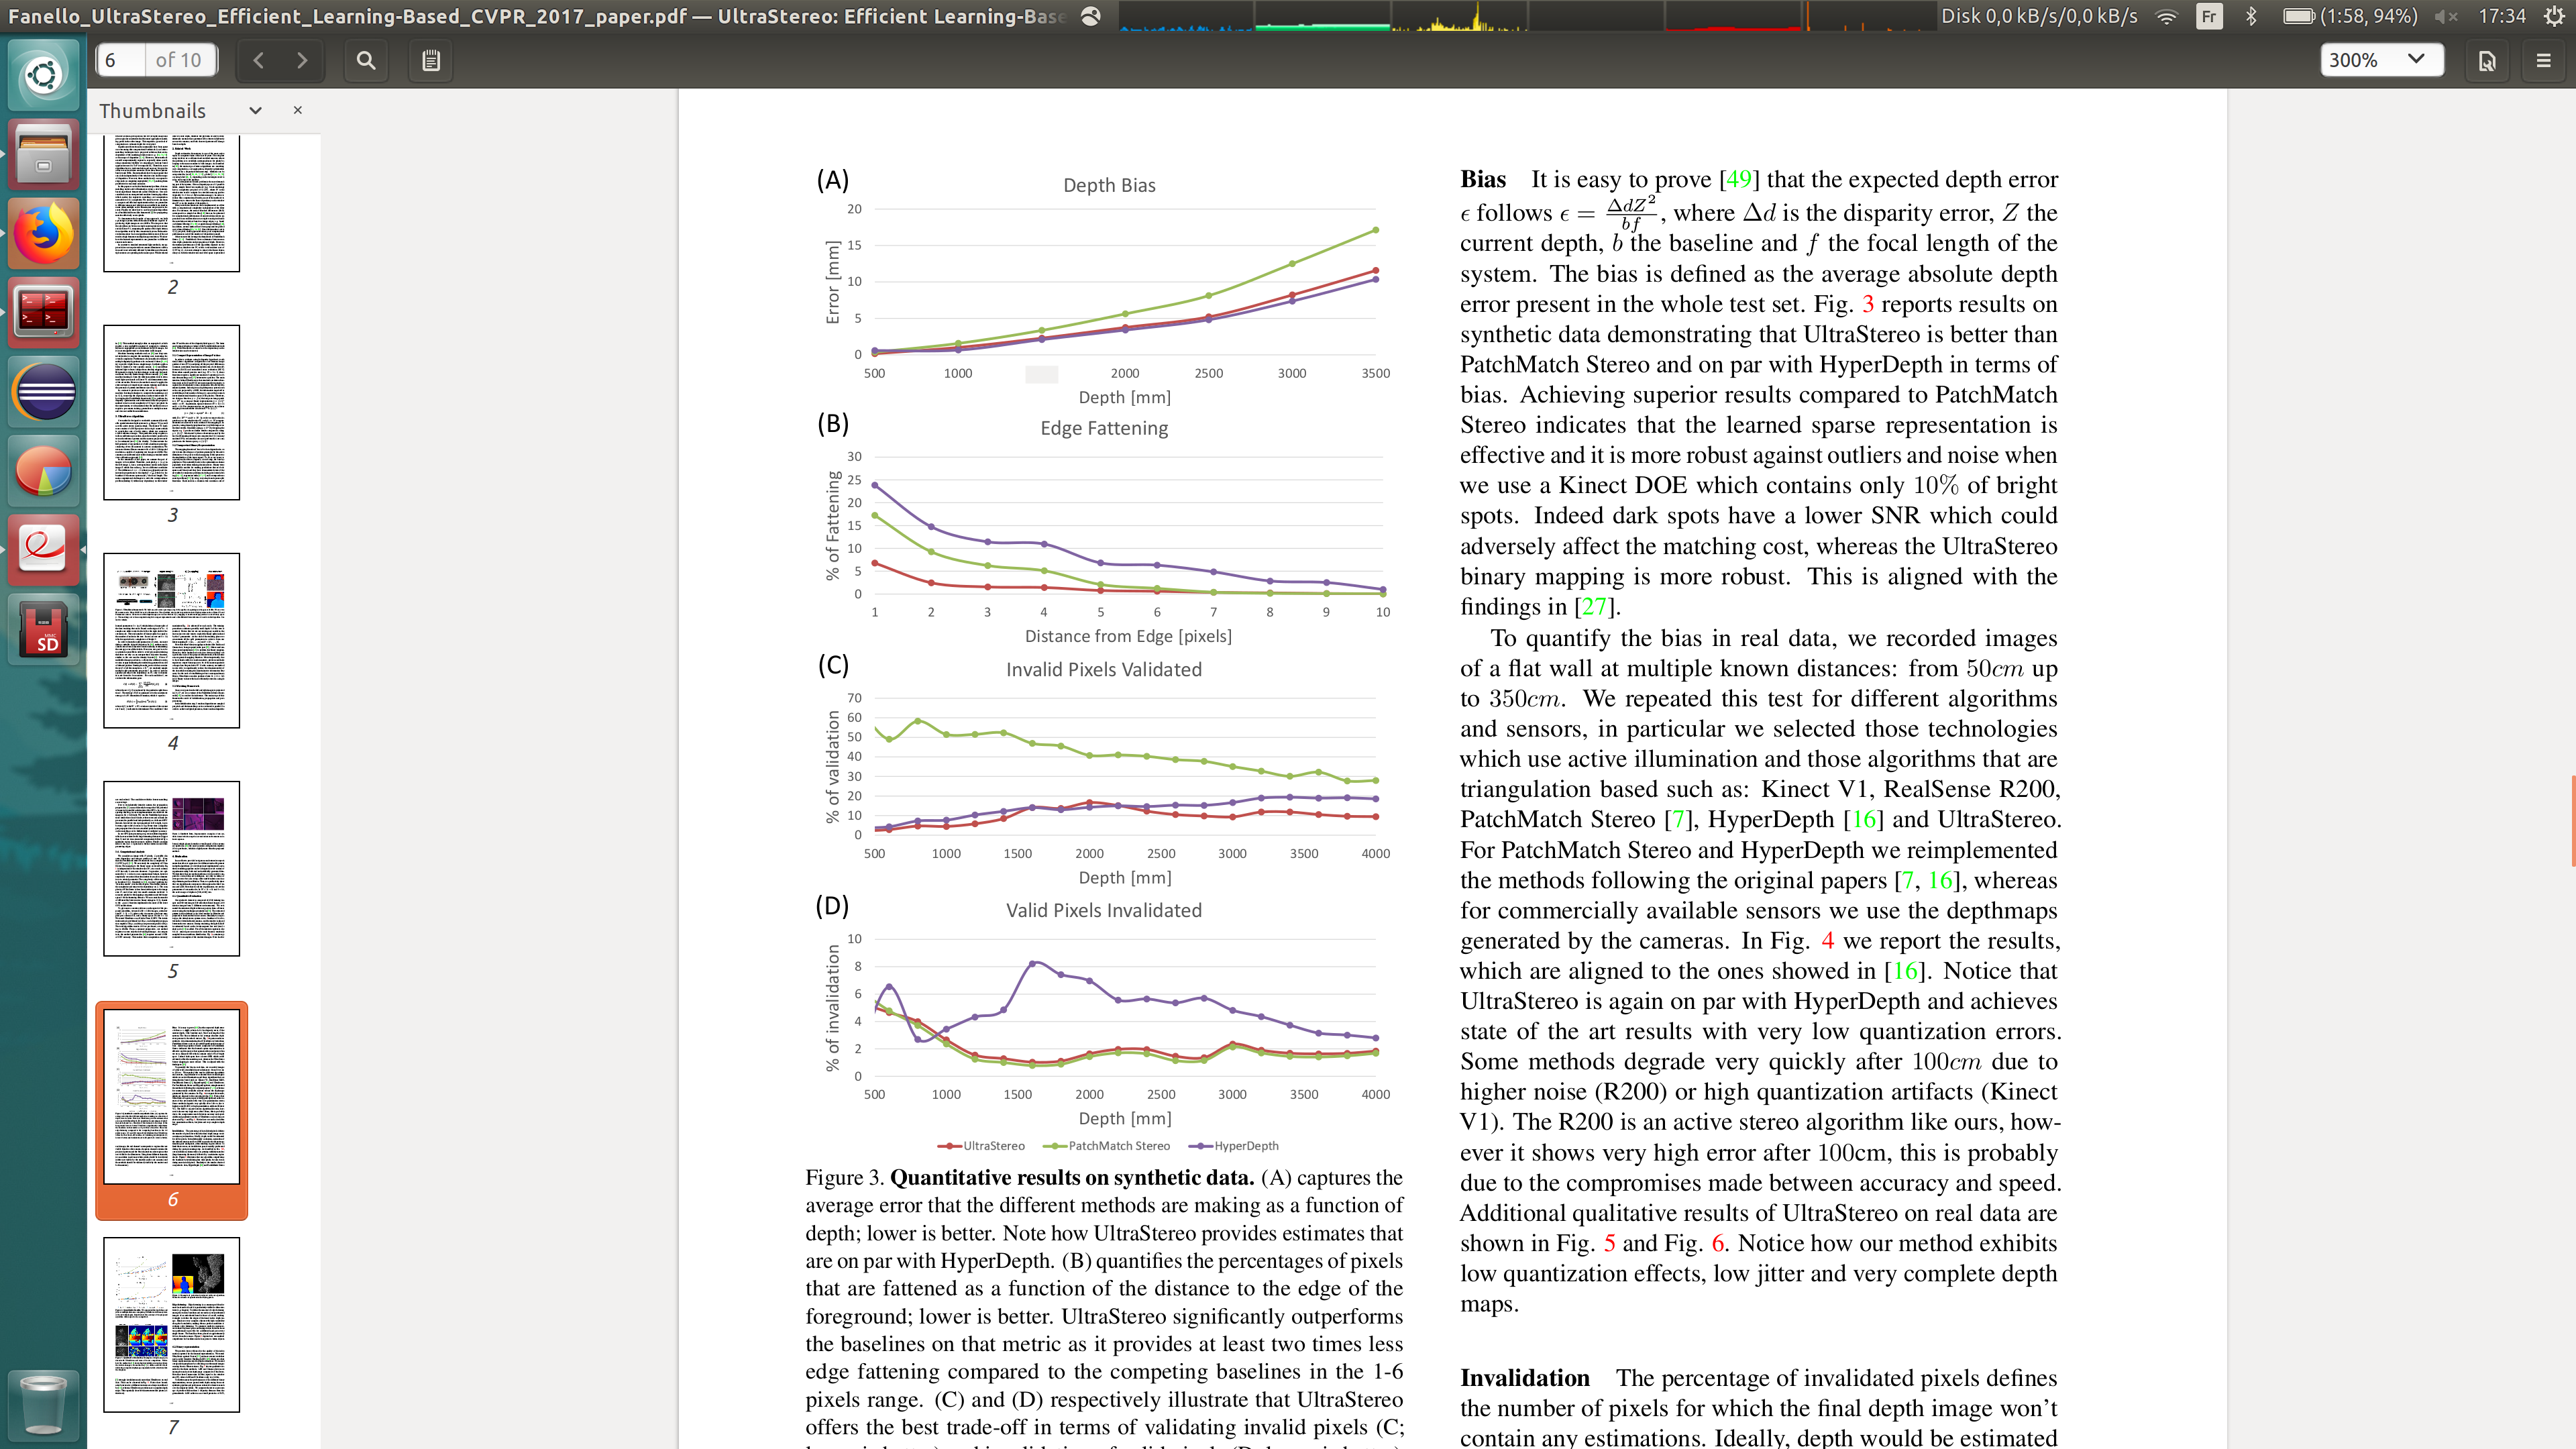
\includegraphics[scale=0.06]{pictures/fig3}
\caption{Quantitative results on syntatic data}
\end{figure}
\end{frame}

\begin{frame}{Edge fattening}

\begin{figure}
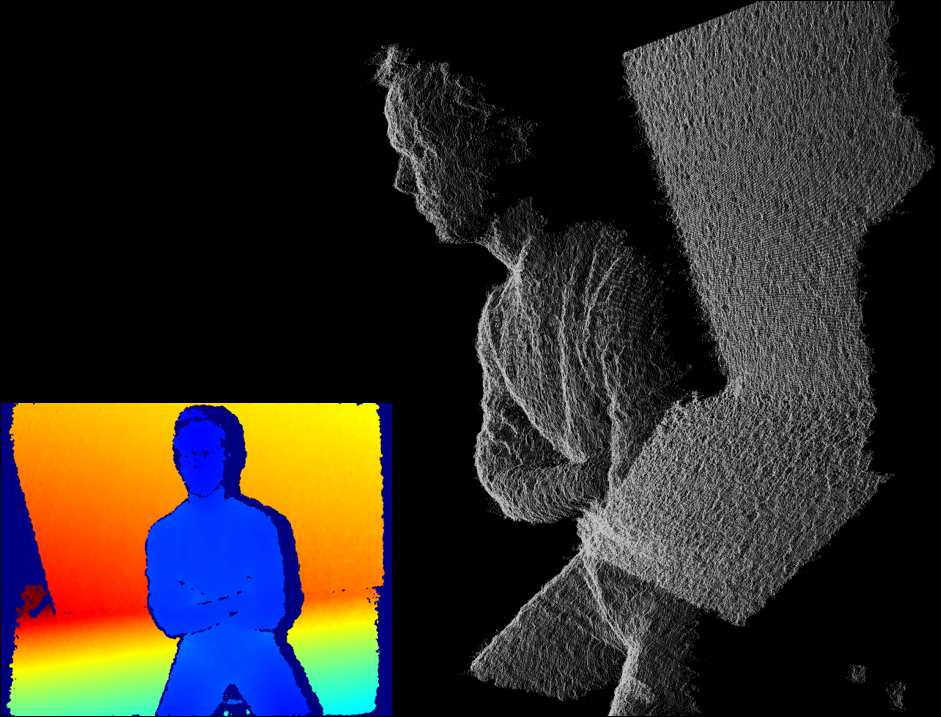
\includegraphics[scale=0.15]{pictures/fig6}
\caption{Example of pointcloud produced with our algorithm. Notice the absence of quantization and flying pixels}
\end{figure}
\end{frame}

\subsection{Binary representation}
\begin{frame}{Binary representation}
\begin{itemize}
\item Compare UltraStereo with Census and Locality Sensitive Hashing (LSH)
\item Collect 1000 images with the Kinnect
\end{itemize}
\begin{figure}
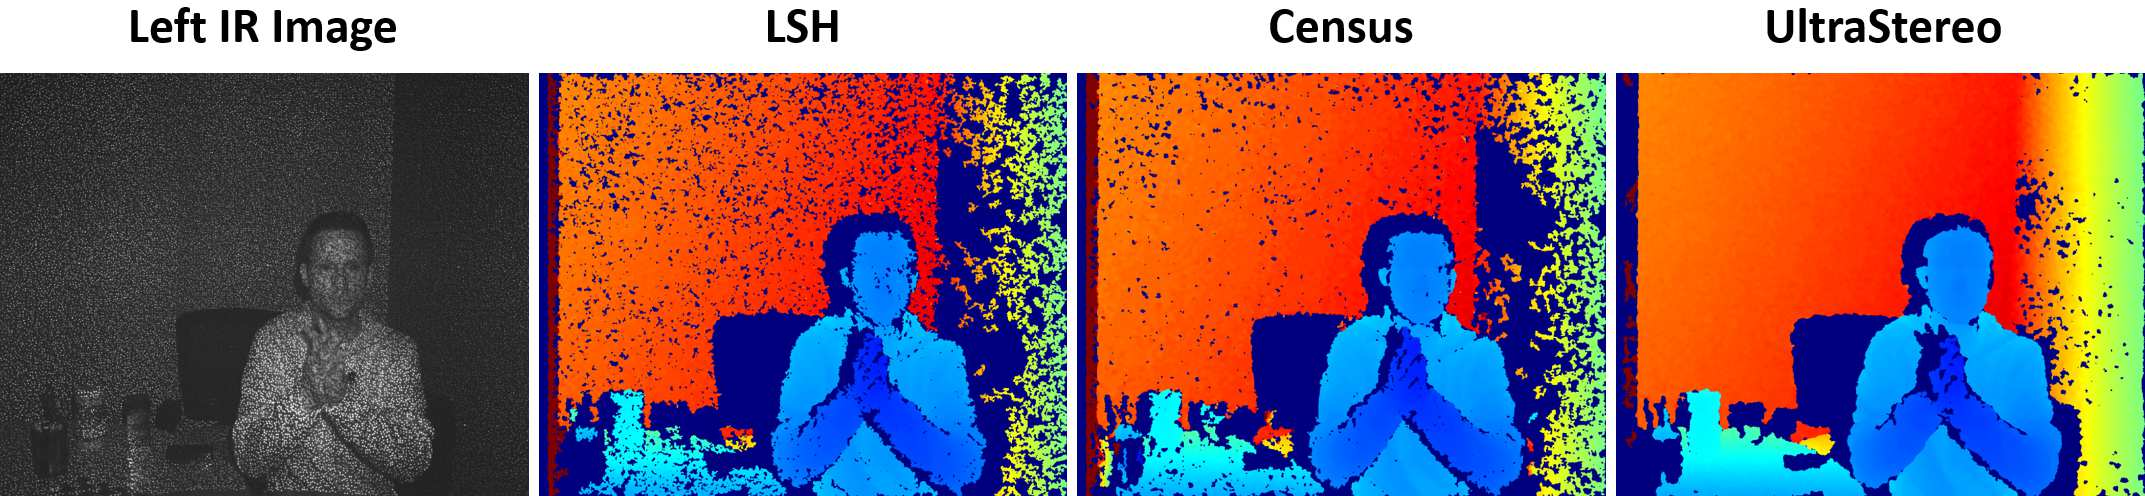
\includegraphics[scale=0.15]{pictures/fig7}
\caption{Census use 121 bits, LSH and UltraStereo use only 32 bits}
\end{figure}
\end{frame}

\subsection{Interference and Generalization}
\begin{frame}{Interference and Generalization}
\begin{itemize}
\item interference caused by multiple sensors
\end{itemize}
\end{frame}

\begin{frame}{Interference and Generalization}
\begin{figure}
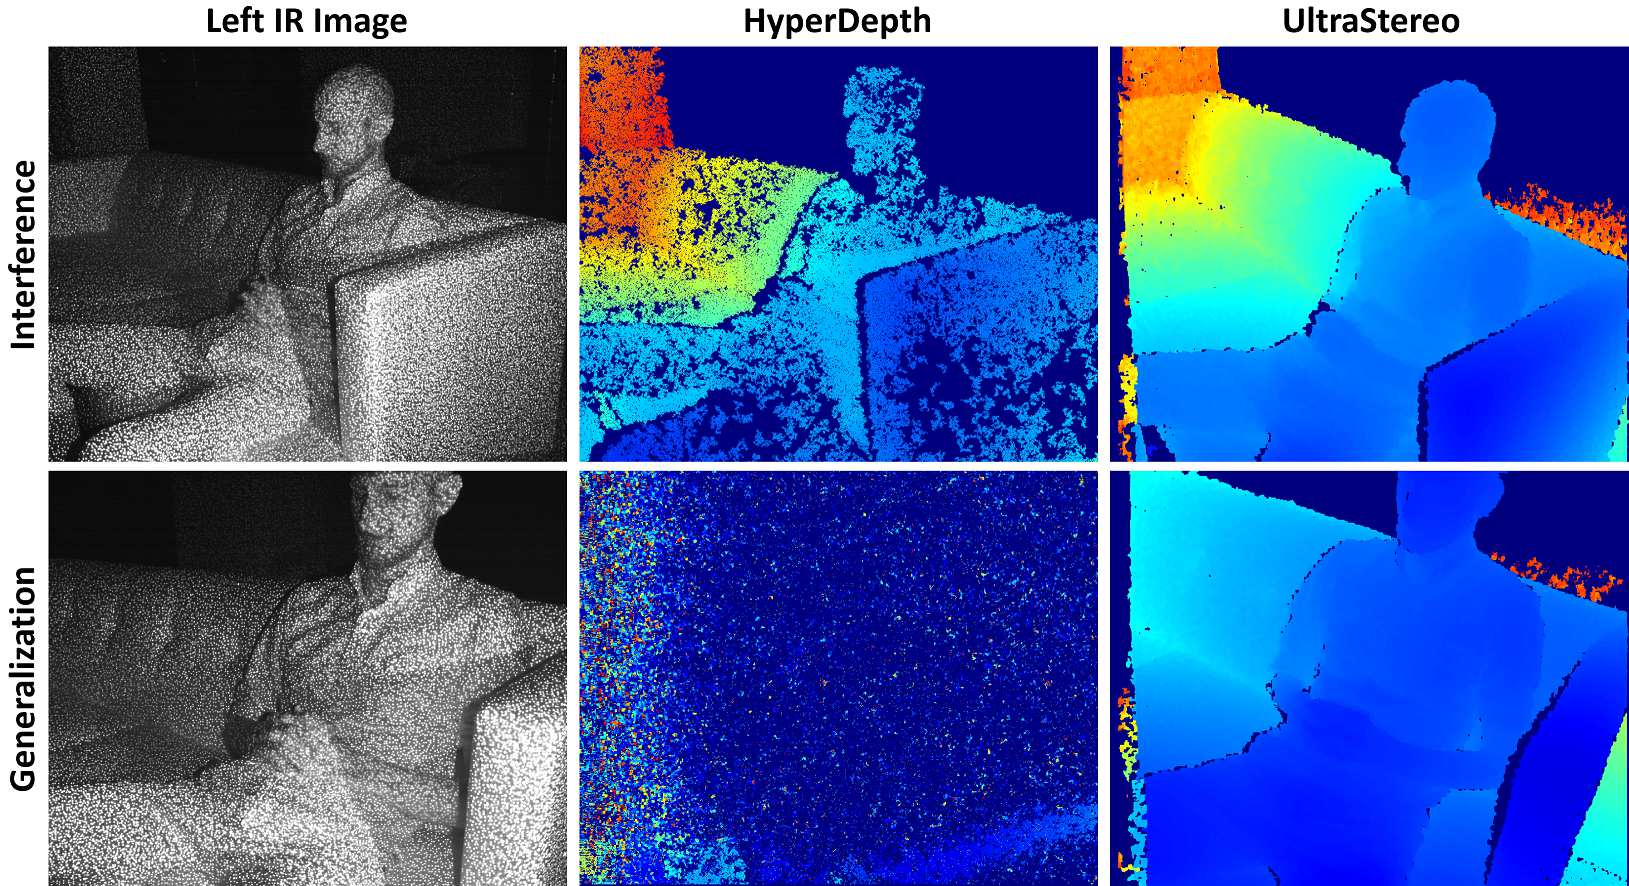
\includegraphics[scale=0.1]{pictures/fig8}
\caption{Examples of depth-maps produced with UltraStereo and state of the art competitors. Notice how the method in shows high invalidation in regions where the texture changes, the method is offline and still it fails delivering complete depth-maps especially in thin structures like the the plant.}
\end{figure}
\end{frame}

\section{Conclusion}
\begin{frame}{Conclusion}
Best algorithms ever made !
From the paper :
\begin{itemize}
\item breakthrough in the field of active stereo depth estimation 
\item does not depend of the e windows size nor the size of the disparity space
\item use machine learning algorithms
\item run on GPU
\item does not suffer from pe camera calibrations nor interference problems
\end{itemize}
\end{frame}
